% Template adapted for Polarization Spectroscopy paper by Joshua Torrance
% 5/11/2015
%%%%%%%%%%%%%%%%%%%%%%% preamble %%%%%%%%%%%%%%%%%%%%%%%%%%%
\documentclass[10pt,letterpaper]{article}
\usepackage{opex3}

%%%%%%%%%%%%%%%%%%%%%%% begin %%%%%%%%%%%%%%%%%%%%%%%%%%%%%%
\begin{document}

%%%%%%%%%%%%%%%%%% title page information %%%%%%%%%%%%%%%%%%
\title{Sub-kilohertz laser linewidth narrowing using polarization spectroscopy}

\author{Joshua S. Torrance,$^{1}$ Ben M. Sparkes,$^1$ Lincoln D. Turner$^2$ and

Robert E. Scholten$^{1*}$}

\address{$^{1}$School of Physics, The University of Melbourne, Victoria 3010 Australia}
\address{$^{2}$School of Physics and Astronomy, Monash University, Victoria 3800 Australia}

%\email{$^*$j.torrance@unimelb.edu.au} %% email address is required
\email{$^*$scholten@unimelb.edu.au} %% email address is required


%%%%%%%%%%%%%%%%%%% abstract and OCIS codes %%%%%%%%%%%%%%%%
\begin{abstract}
We identify several beneficial characteristics of polarization spectroscopy as an absolute atomic reference for frequency stabilization of lasers, and demonstrate sub-kilohertz laser spectral linewidth narrowing using polarization spectroscopy with high-bandwidth feedback.
Polarization spectroscopy provides a highly dispersive velocity-selective absolute atomic reference based on frequency-dependent birefringence in an optically pumped atomic gas.
The pumping process leads to dominance of the primary closed transition, suppressing closely-spaced subsidiary resonances which reduce the effective capture range for conventional atomic references.
The locking signal is based on subtraction of two orthogonal polarization signals, reducing the effect of laser intensity noise to the shot noise limit.
We measure noise-limited servo bandwidth comparable to that of a high-finesse optical cavity without the frequency limit or complexity imposed by optical modulation normally associated with high bandwidth laser frequency stabilization.
We demonstrate narrowing to 600$\pm$100\,Hz laser linewidth using the beatnote between two similarly locked external cavity diode lasers.
\end{abstract}

\ocis{(140.3425) Laser stabilization; (300.6210) Spectroscopy, atomic.} % REPLACE WITH CORRECT OCIS CODES FOR YOUR ARTICLE, MINIMUM OF TWO; Avoid using the OCIS codes for “General” or “General science” whenever possible.

%%%%%%%%%%%%%%%%%%%%%%% References %%%%%%%%%%%%%%%%%%%%%%%%%
\begin{thebibliography}{10}
\newcommand{\enquote}[1]{``#1''}

\bibitem{uetake_high_2008}
S.~Uetake, A.~Yamaguchi, S.~Kato, and Y.~Takahashi, \enquote{High power narrow
  linewidth laser at 556\,nm for magneto-optical trapping of ytterbium,} Applied
  Physics B \textbf{92}, 33--35 (2008).

\bibitem{ye_stable_2010}
L.~Ye, L.~Yi-Ge, Z.~Yang, W.~Qiang, W.~Shao-Kai, Y.~Tao, C.~Jian-Ping,
  L.~Tian-Chu, F.~Zhan-Jun, and Z.~Er-Jun, \enquote{Stable narrow linewidth
  689\,nm diode laser for the second stage cooling and trapping of
  strontium atoms,} Chinese Physics Letters \textbf{27}, 074208 (2010).

\bibitem{akamatsu_narrow_2012}
D.~Akamatsu, Y.~Nakajima, H.~Inaba, K.~Hosaka, M.~Yasuda, A.~Onae, and F.-L.
  Hong, \enquote{Narrow linewidth laser system realized by linewidth transfer
  using a fiber-based frequency comb for the magneto-optical trapping of
  strontium,} Optics Express \textbf{20}, 16010 (2012).

\bibitem{anderson_observation_1995}
M.~H. Anderson, J.~R. Ensher, M.~R. Matthews, C.~E. Wieman, and E.~A. Cornell,
  \enquote{Observation of {Bose}-{Einstein} condensation in a dilute
  atomic vapor,} Science \textbf{269}, 198--201 (1995).

\bibitem{demarco_onset_1999}
B.~DeMarco and D.~S. Jin, \enquote{Onset of {Fermi} degeneracy in a trapped
  atomic gas,} Science \textbf{285}, 1703--1706 (1999).

\bibitem{ludlow_sr_2008}
A.~D. Ludlow, T.~Zelevinsky, G.~K. Campbell, S.~Blatt, M.~M. Boyd, M.~H. G.~de
  Miranda, M.~J. Martin, J.~W. Thomsen, S.~M. Foreman, J.~Ye, T.~M. Fortier,
  J.~E. Stalnaker, S.~A. Diddams, Y.~L. Coq, Z.~W. Barber, N.~Poli, N.~D.
  Lemke, K.~M. Beck, and C.~W. Oates, \enquote{Sr lattice clock at $1\times10^{-16}$
  fractional uncertainty by remote optical evaluation with a Ca clock,} Science \textbf{319}, 1805--1808 (2008).

\bibitem{rafac_sub-dekahertz_2000}
R.~J. Rafac, B.~C. Young, J.~A. Beall, W.~M. Itano, D.~J. Wineland, and J.~C.
  Bergquist, \enquote{Sub-dekahertz ultraviolet spectroscopy of $^{199}$Hg$^+$,}
  Physical Review Letters \textbf{85}, 2462--2465 (2000).

\bibitem{metcalf_laser_1999}
H.~J. Metcalf and P.~van~der Straten, \emph{Laser cooling and trapping}
  (Springer, 1999).

\bibitem{ye_quantum_2008}
J.~Ye, H.~J. Kimble, and H.~Katori, \enquote{Quantum state engineering and
  precision metrology using state-insensitive light traps,}
  Science \textbf{320}, 1734--1738 (2008).

\bibitem{maguire_theoretical_2006}
L.~P. Maguire, R.~M. W.~van Bijnen, E.~Mese, and R.~E. Scholten,
  \enquote{Theoretical calculation of saturated absorption spectra for
  multi-level atoms,} Journal of Physics B: Atomic, Molecular and Optical
  Physics \textbf{39}, 2709--2720 (2006).

\bibitem{haroche_theory_1972}
S.~Haroche and F.~Hartmann, \enquote{Theory of saturated-absorption line
  shapes,} Physical Review A \textbf{6}, 1280--1300 (1972).

\bibitem{preston_doppler-free_1996}
D.~W. Preston, \enquote{Doppler-free saturated absorption: Laser
  spectroscopy,} American Journal of Physics \textbf{64}, 1432 (1996).

\bibitem{cuneo_optically_1994}
C.~J. Cuneo, J.~J. Maki, and D.~H. McIntyre, \enquote{Optically stabilized
  diode laser using high-contrast saturated absorption,} Applied Physics
  Letters \textbf{64}, 2625--2627 (1994).

\bibitem{saliba_linewidths_2009}
S.~D. Saliba and R.~E. Scholten, \enquote{Linewidths below 100\,kHz with
  external cavity diode lasers,} Applied Optics \textbf{48}, 6961 (2009).

\bibitem{drever_laser_1983}
R.~Drever, J.~L. Hall, F.~Kowalski, J.~Hough, G.~Ford, A.~Munley, and H.~Ward,
  \enquote{Laser phase and frequency stabilization using an optical resonator,}
  Applied Physics B \textbf{31}, 97--105 (1983).

\bibitem{ludlow_compact_2007}
A.~D. Ludlow, X.~Huang, M.~Notcutt, T.~Zanon-Willette, S.~M. Foreman, M.~M.
  Boyd, S.~Blatt, and J.~Ye, \enquote{Compact, thermal-noise-limited optical
  cavity for diode laser stabilization at $1\times10^{\textrm{-15}}$,} Optics
  Letters \textbf{32}, 641 (2007).
  
\bibitem{hansch_laser_1980}
H\"ansch, T. W. and Couillaud, B., \enquote{Laser frequency stabilization by
  polarization spectroscopy of a reflecting reference cavity,}
  Optics Communications \textbf{35}, 441--444 (1980).

\bibitem{tiltlock}
D.~A.~Shaddock, M.~B.~Gray,and D.~E.~McClelland,
\enquote{Frequency locking a laser to an optical cavity by use of spatial mode interference},
Optics Letters \textbf{24}, 1499 (1999).

\bibitem{robins_Interferometric_2002}
N.~P. Robins, B.~J.~J. Slagmolen, D.~A. Shaddock, J.~D. Close, and M.~B. Gray,
  \enquote{Interferometric, modulation-free laser stabilization,} Optics
  Letters \textbf{27}, 1905 (2002).

\bibitem{corwin_frequency-stabilized_1998}
K.~L. Corwin, Z.-T. Lu, C.~F. Hand, R.~J. Epstein, and C.~E. Wieman,
  \enquote{Frequency-stabilized diode laser with the Zeeman shift in
  an atomic vapor,} Applied Optics \textbf{37}, 3295--3298 (1998).

\bibitem{millett-sikking_davll_2007}
A.~Millett-Sikking, I.~G. Hughes, P.~Tierney, and S.~L. Cornish,
  \enquote{{DAVLL} lineshapes in atomic rubidium,} Journal of Physics B:
  Atomic, Molecular and Optical Physics \textbf{40}, 187 (2007).

\bibitem{shirley_modulation_1982}
J.~H. Shirley, \enquote{Modulation transfer processes in optical heterodyne
  saturation spectroscopy,} Optics Letters \textbf{7}, 537 (1982).

\bibitem{mccarron_modulation_2008}
D.~J. McCarron, S.~A. King, and S.~L. Cornish, \enquote{Modulation transfer
  spectroscopy in atomic rubidium,} Measurement Science and Technology
  \textbf{19}, 105601 (2008).

\bibitem{negnevitsky_wideband_2013}
V.~Negnevitsky and L.~D. Turner, \enquote{Wideband laser locking to an atomic
  reference with modulation transfer spectroscopy,} Optics Express \textbf{21},
  3103 (2013).

\bibitem{jundt_non-linear_2003}
G.~Jundt, G.~T. Purves, C.~S. Adams, and I.~G. Hughes, \enquote{Non-linear
  {Sagnac} interferometry for pump-probe dispersion spectroscopy,} The European
  Physical Journal D - Atomic, Molecular, Optical and Plasma Physics
  \textbf{27}, 273--276 (2003).

\bibitem{wieman_doppler-free_1976}
C.~Wieman and T.~W. H\"ansch, \enquote{Doppler-free laser polarization
  spectroscopy,} Physical Review Letters \textbf{36}, 1170--1173 (1976).

\bibitem{demtroder_laser_2003}
W.~Demtr\"oder, \emph{Laser spectroscopy: Basic concepts and
  Instrumentation} (Springer Science \& Business Media, 2003).
  
\bibitem{torii_laser-phase_2012}
Y.~Torii, H.~Tashiro, N.~Ohtsubo, and T.~Aoki, \enquote{Laser-phase and
  frequency stabilization using atomic coherence,} Physical Review A
  \textbf{86}, 033805 (2012).

\bibitem{yoshikawa_frequency_2003}
Y.~Yoshikawa, T.~Umeki, T.~Mukae, Y.~Torii, and T.~Kuga, \enquote{Frequency
  stabilization of a laser diode with use of light-induced
  birefringence in an atomic vapor,} Applied Optics \textbf{42}, 6645
  (2003).

\bibitem{pearman_polarization_2002}
C.~P. Pearman, C.~S. Adams, S.~G. Cox, P.~F. Griffin, D.~A. Smith, and I.~G.
  Hughes, \enquote{Polarization spectroscopy of a closed atomic transition:
  applications to laser frequency locking,} Journal of Physics B: Atomic,
  Molecular and Optical Physics \textbf{35}, 5141 (2002).

\bibitem{hughes_polarization_2009}
I.~G. Hughes, \enquote{Polarization spectroscopy of alkali-metal
  atoms,} New Trends in Quantum Coherence and Nonlinear Optics \textbf{263},
  149--169 (2009).

\bibitem{equipment}
Lasers: MOGLabs ECD003 and Toptica DL pro. Laser Controllers: MOGLabs DLC 202
  and DLC 252, Servo-controllers: NewFocus LB1005. PS Photodectors: Thorlabs
  PDA10A. Cavity Photodetector: Thorlabs PDA36A-EC. Heterodyne Photodetector:
  NewFocus 1621. Optical Cavity: Stable Laser Systems. Spectrum Analyzer:
  Rohde \& Schwarz FSP7. Audio digitizer: E-Mu E-DSP. Certain commercial
  equipment, instruments, or materials are identified in this paper in order
  to adequately specify the experimental procedure. Such identification does
  not imply recommendation or endorsement, nor does it imply that the
  materials or equipment are necessarily the best available for the purpose.

\bibitem{wiemanhollberg}
C.~E.~Wieman and L.~Hollberg, \enquote{Using diode lasers for atomic physics},
Review of Scientific Instruments \textbf{62}, 1--20 (1991).

\bibitem{tiwari_laser_2006}
V.~B. Tiwari, S.~Singh, S.~R. Mishra, H.~S. Rawat, and S.~C. Mehendale,
  \enquote{Laser frequency stabilization using {Doppler}-free bi-polarization
  spectroscopy,} Optics Communications \textbf{263}, 249--255 (2006).

\bibitem{lee_frequency_2014}
M.~W. Lee, M.~C. Jarratt, C.~Marciniak, and M.~J. Biercuk, \enquote{Frequency
  stabilization of a 369\,nm diode laser by nonlinear spectroscopy of
  ytterbium ions in a discharge,} Optics Express \textbf{22}, 7210
  (2014).

\end{thebibliography}

%%%%%%%%%%%%%%%%%%%%%%%%%%  body  %%%%%%%%%%%%%%%%%%%%%%%%%%

\section{Introduction}

Laser frequency stabilization to atomic references is essential to numerous applications including the cooling and trapping of atoms~\cite{uetake_high_2008, ye_stable_2010, akamatsu_narrow_2012}, Bose-Einstein condensates~\cite{anderson_observation_1995} and degenerate Fermi gases~\cite{demarco_onset_1999}.
Stabilization techniques that provide high-bandwidth feedback can allow narrowing of the laser spectral linewidth, which is important to applications such as atomic clocks~\cite{ludlow_sr_2008}, high resolution spectroscopy~\cite{rafac_sub-dekahertz_2000} and metrology~\cite{metcalf_laser_1999, ye_quantum_2008}.

The desirable traits of a laser frequency stabilization scheme include reference to an absolute atomic transition, high bandwidth to achieve low spectral linewidth, long-term stability, and low complexity in particular the absence of laser beam frequency or amplitude modulation.
Established techniques range from saturated absorption spectroscopy (SA)~\cite{maguire_theoretical_2006, haroche_theory_1972, preston_doppler-free_1996}, which can reduce external cavity diode laser (ECDL) linewidth below 100\,kHz~\cite{cuneo_optically_1994, saliba_linewidths_2009}, to high-finesse optical cavities that are able to achieve sub-Hertz linewidth~\cite{drever_laser_1983,ludlow_compact_2007}.
Optical cavity techniques use the Pound-Drever-Hall (PDH) technique~\cite{drever_laser_1983} with laser modulation, polarization dependent dispersion~\cite{hansch_laser_1980} or spatial mode interference~\cite{tiltlock}, but require a secondary mechanism for absolute frequency stability~\cite{robins_Interferometric_2002}.

Inherently absolute frequency stabilization methods based on atomic references include SA, dichroic atomic vapor laser lock~\cite{corwin_frequency-stabilized_1998,millett-sikking_davll_2007}, modulation transfer spectroscopy (MTS)~\cite{shirley_modulation_1982,mccarron_modulation_2008,negnevitsky_wideband_2013}, Sagnac interferometry~\cite{robins_Interferometric_2002,jundt_non-linear_2003} and polarization spectroscopy (PS)~\cite{wieman_doppler-free_1976, demtroder_laser_2003}.

It has been shown recently that PS can achieve an effective servo bandwidth comparable to PDH with a high-finesse optical cavity~\cite{torii_laser-phase_2012,yoshikawa_frequency_2003}, yet with complexity comparable to SA; that is, with a simple atomic gas cell and without requiring amplitude or frequency modulation.
The full width at half maximum (FWHM) linewidth of a distributed feedback diode was reduced to 20\,kHz~\cite{torii_laser-phase_2012} and of an ECDL to 65\,kHz~\cite{yoshikawa_frequency_2003}.

Here we demonstrate sub-kilohertz linewidth narrowing using PS, measured with a high-finesse optical cavity and heterodyne measurement between two similar lasers.
We review the characteristics of PS that enable such high bandwidth noise suppression, and the potential for further improvement.

\section{Polarization Spectroscopy}

A schematic diagram for PS is shown in Fig.~\ref{fig:polspec_schematic}.
A circularly polarized pump beam from a monochromatic laser induces frequency-dependent circular birefringence in a magnetically-shielded atomic gas sample.
A linearly polarized beam from the same source is used to measure the birefringence, monitored with a balanced polarimeter consisting of a half-wave phase retarder, polarizing beam splitter (PBS) and two detectors.
The dispersive error signal is the difference of the two orthogonal polarization components~\cite{pearman_polarization_2002, hughes_polarization_2009}
\begin{equation}
P_{PS} = P_x-P_y = -P_0 \cos(2\phi+2\Phi)\label{P_PS}
\end{equation}
where $P_{x,y}$ are the power of the horizontal and vertical linearly polarized components of the probe after the sample, $P_0$ is the power of the probe in the absence of a pump beam, $\phi$ is the angle of polarization of the probe in the absence of a pump beam and $\Phi$ is the additional polarization rotation of the probe due to the birefringence induced by the pump.
The largest PS spectrum is produced when $\phi=\pi/4$ and since $\Phi$ is small Eq.~(\ref{P_PS})  becomes
\begin{equation}
P_{PS} = 2P_0 \Phi.
\end{equation}
The polarization rotation is given by
\begin{equation}
\Phi = \frac{\pi L \Delta n}{\lambda},
\end{equation}
where $L$ is the length of the atomic sample, $\lambda$ is the wavelength of the light, $\Delta n = n_+ - n_-$ and $n_\pm$ are the refractive indices affecting the circularly polarized components of the probe beam.
\begin{figure}[htbp]
\centering
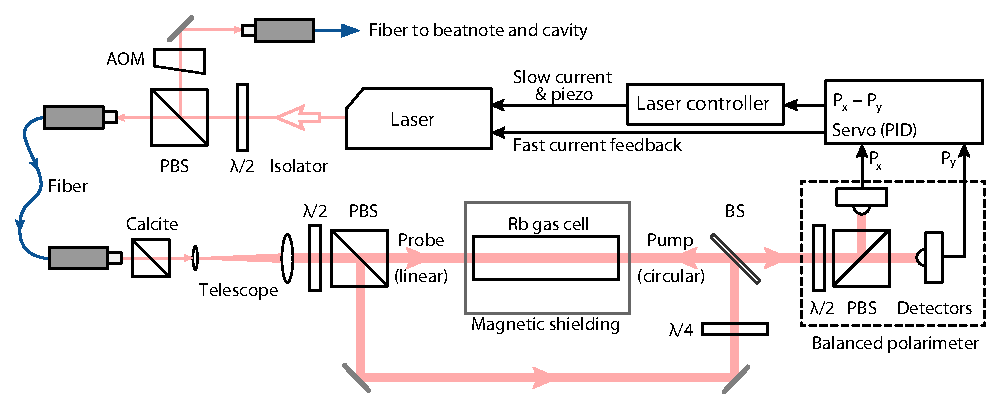
\includegraphics[width=\linewidth]{scholten_fig1.pdf}
\caption{Schematic of polarization spectroscopy (PS) apparatus.
The beam from the laser passes through an isolator before being split into two beams by a polarizing beam splitter (PBS) and coupled into optical fibers.
One fiber leads to the PS setup shown here, the other to measurement or experimental apparatus via an acousto-optic modulator (AOM).
The PS setup  consists of a polarization stabilizing Glan-Thompson prism followed by a beam expanding telescope.
The expanded beam is then divided by a PBS into a linearly polarized probe and circularly polarized pump which counter-propagate, via a non-polarizing 50:50 beam splitter (BS), through the magnetically shielded atomic gas sample.
The polarization rotation of the probe beam is then measured by a balanced polarimeter which consists of a $\lambda/2$ waveplate, PBS and two photodetectors.\label{fig:polspec_schematic}}
\end{figure}

The refractive index and absorption of the medium are related through the Kramers-Kronig dispersion relation to give~\cite{demtroder_laser_2003}
\begin{equation}
\Delta n = \Delta\alpha_0 \frac{2c}{\omega_A \Gamma}\frac{\delta}{1+4\left(\frac{\delta}{\Gamma}\right)^2}.\label{result}
\end{equation}
Here $c$ is the speed of light, $\delta=\omega_L-\omega_A$ is the detuning of the laser from the resonance, $\omega_{L,\,A}$ are the angular frequency of the laser and the atomic resonance, and $\Gamma$ is the inverse lifetime of the excited state of the resonant transition.
$\Delta\alpha_0$ is the difference in absorption coefficients for the circular polarization components at zero detuning.
$\Delta\alpha_0$ is the sum over all $m_F$ ground states of the difference between absorption coefficients for each circular polarization, with $\delta=0$, weighted by the ground and excited state population differences, $\mathcal{P}_{F,m_F}-\mathcal{P}_{F',m_{F\pm1}}$;
\begin{eqnarray}
\Delta\alpha_0 &=& \sum_{m_F=-F}^{+F} \big[\alpha_{(F,m_F\rightarrow F',m_{F+1})}(\mathcal{P}_{F,m_F}-\mathcal{P}_{F',m_{F+1}})\nonumber\\
&&-\alpha_{(F,m_F\rightarrow F',m_{F-1})}(\mathcal{P}_{F,m_F}-\mathcal{P}_{F',m_{F-1}})\big].
\end{eqnarray}
The absorption coefficient for a given transition is $\alpha_{(F, m_F\rightarrow F',m_{F\pm1})}=N \sigma(\omega_L)$ where $N$ is the total number of interacting atoms, and $\sigma(\omega_L)$ is the absorption cross section for the transition.

The atomic substate populations established by interaction with the pump beam can be calculated using optical Bloch equations~\cite{hughes_polarization_2009}.
The PS signal is proportional to the refractive index difference given by Eq.~(\ref{result}), which describes a steep, background-free antisymmetric dispersive function.

\section{Signal characteristics}
Several characteristics of the dispersive PS signal contribute to a high servo locking bandwidth.

\subsection{High signal-to-noise ratio}
PS is velocity selective, producing dispersive error signals with high frequency discrimination slope, comparable to SA and MTS.
The subtraction associated with the balanced polarimeter of PS removes technical noise, particularly probe laser intensity noise, across the entire signal bandwidth.
The resulting PS dispersion signal therefore approaches the shot-noise limit, and the signal-to-noise ratio is very high over a large bandwidth.

\subsection{Modulation free}
PS is modulation-free; that is, a baseband technique.
With modulation-based methods such as PDH, FM demodulation used with SA, and MTS, the feedback bandwidth is limited in theory by the Nyquist limit of half the modulation frequency but in practice to well below this due to the need for a filter to remove the second harmonic product and upconverted flicker noise at the first harmonic, made more difficult in servo applications by the need to keep latency low to preserve phase margin.
The absence of modulation also reduces complexity and cost, but some care is needed to minimize noise contributions at very low frequencies which contribute to frequency drift, and at high frequencies where noise may exceed the signal.

\subsection{Selectivity}
PS optically pumps the atomic sample into the primary transition pair, for example the $5^2S_{1/2} F=3\rightarrow5^2P_{3/2} F=4$ transition with $^{85}$Rb.
Subsidiary transitions such as $F=3\rightarrow F=3$ are strongly suppressed and the cross-over resonances of SA are relatively small and do not cross zero.
This selectivity, which also applies to MTS, has two important benefits.
First, the PS signal is of the correct sign over the full Doppler width of the sample, free of zero-crossings at nearby secondary resonances, allowing for a high effective feedback bandwidth.
Second, if a laser locked to the PS feature becomes unlocked, for example due to external disturbance, there are no zero-crossings in the feedback error signal to trap the locking servo except at the desired primary transition.
\\
\\
Collectively, these characteristics show that PS has excellent prospects for application as a wide-bandwidth linewidth-narrowing frequency stabilization reference linked to an absolute atomic transition.
Our experiments separately demonstrate these characteristics and show that the sensitivity to low-frequency drift and high-frequency noise can be mitigated.

\section{Experiment}
Two commercial Littrow configuration ECDLs~\cite{equipment} were individually locked using PS.
The laser beam for each was split by a PBS and propagated through polarization-maintaining fibers to the PS locking system and linewidth measurements.
The locking beams were polarized with Glan-Thompson prisms to eliminate residual polarization drift in the fibers.
Beam-expanding telescopes were used to expand the beam to fill the apertures of the magnetic shielding, 1.5\,cm diameter, reducing power broadening and improving the optical pumping.

The balanced polarimeter error signal was generated with biased photodiodes (150\,MHz bandwidth) and servo controllers (14\,MHz bandwidth).
The servo controller integration zero-gain frequency was typically between 100\,kHz and 1\,MHz.
The feedback to the diode injection current could be DC-coupled or AC-coupled, with DC (AC) bandwidths of 40\,MHz (100\,kHz\,\textendash\,40\,MHz) and 10\,MHz (10\,kHz\,\textendash\,10\,MHz) for the two lasers.
Laser electronics provided control of each ECDL piezoelectric transducer and diode injection current, with bandwidths of 1\,kHz and 50\,kHz respectively.

\section{Results} \label{results_section}

We have characterized the spectral linewidth of the locked lasers using high-finesse optical cavity transmission and heterodyne techniques, the frequency noise spectra of the locked lasers, and the long-term frequency stability of the locked lasers.

\subsection{Polarization Spectroscopy Capture Range}\label{bandwidth_section}
The capture range of the frequency discriminator is important in determining the ability to compensate for sudden disturbances to the laser frequency, for example due to external shock or vibration.
We define the capture range as the range of frequencies about the resonance for which the error signal is of the correct sign to provide negative feedback.
This can be deduced from the error signal by locating the first zero crossing to either side of the resonance.
For the spectra shown in Fig.~\ref{fig:sa_ps_spectra} the capture range is greater than $\pm 150\rm\,MHz$, many times larger than the $\pm 15\rm\,MHz$ of SA.

\begin{figure}[htbp]
    \centering
    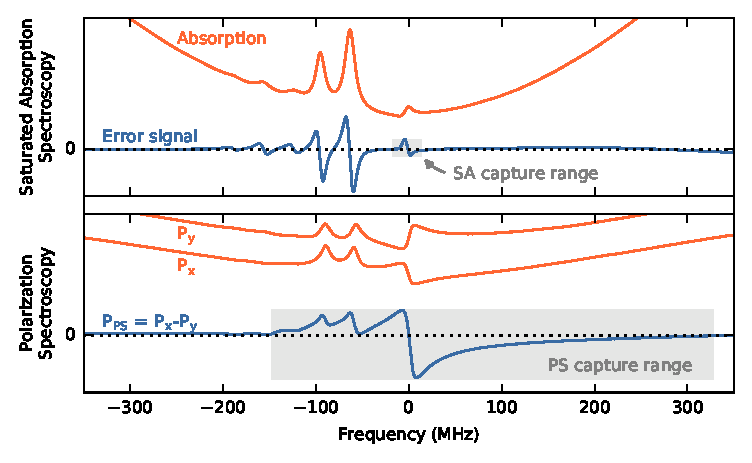
\includegraphics{scholten_fig2.pdf}
    \caption{Saturated absorption spectroscopy (SA, upper) and polarization spectroscopy (PS, lower) absorption and error spectra for the $^{85}$Rb D2 transition.
    The components of the PS error signal ($P_{x,y}$) are also shown.
    The shaded regions indicate the approximate capture range of the respective error signals.
    Zero frequency corresponds to the $^{85}$Rb, $5^2S_{1/2} F=3\rightarrow5^2P_{3/2} F=4$ transition.\label{fig:sa_ps_spectra}}
\end{figure}    

\subsection{Frequency Noise Measurements}

\begin{figure}[htbp]
\centering
    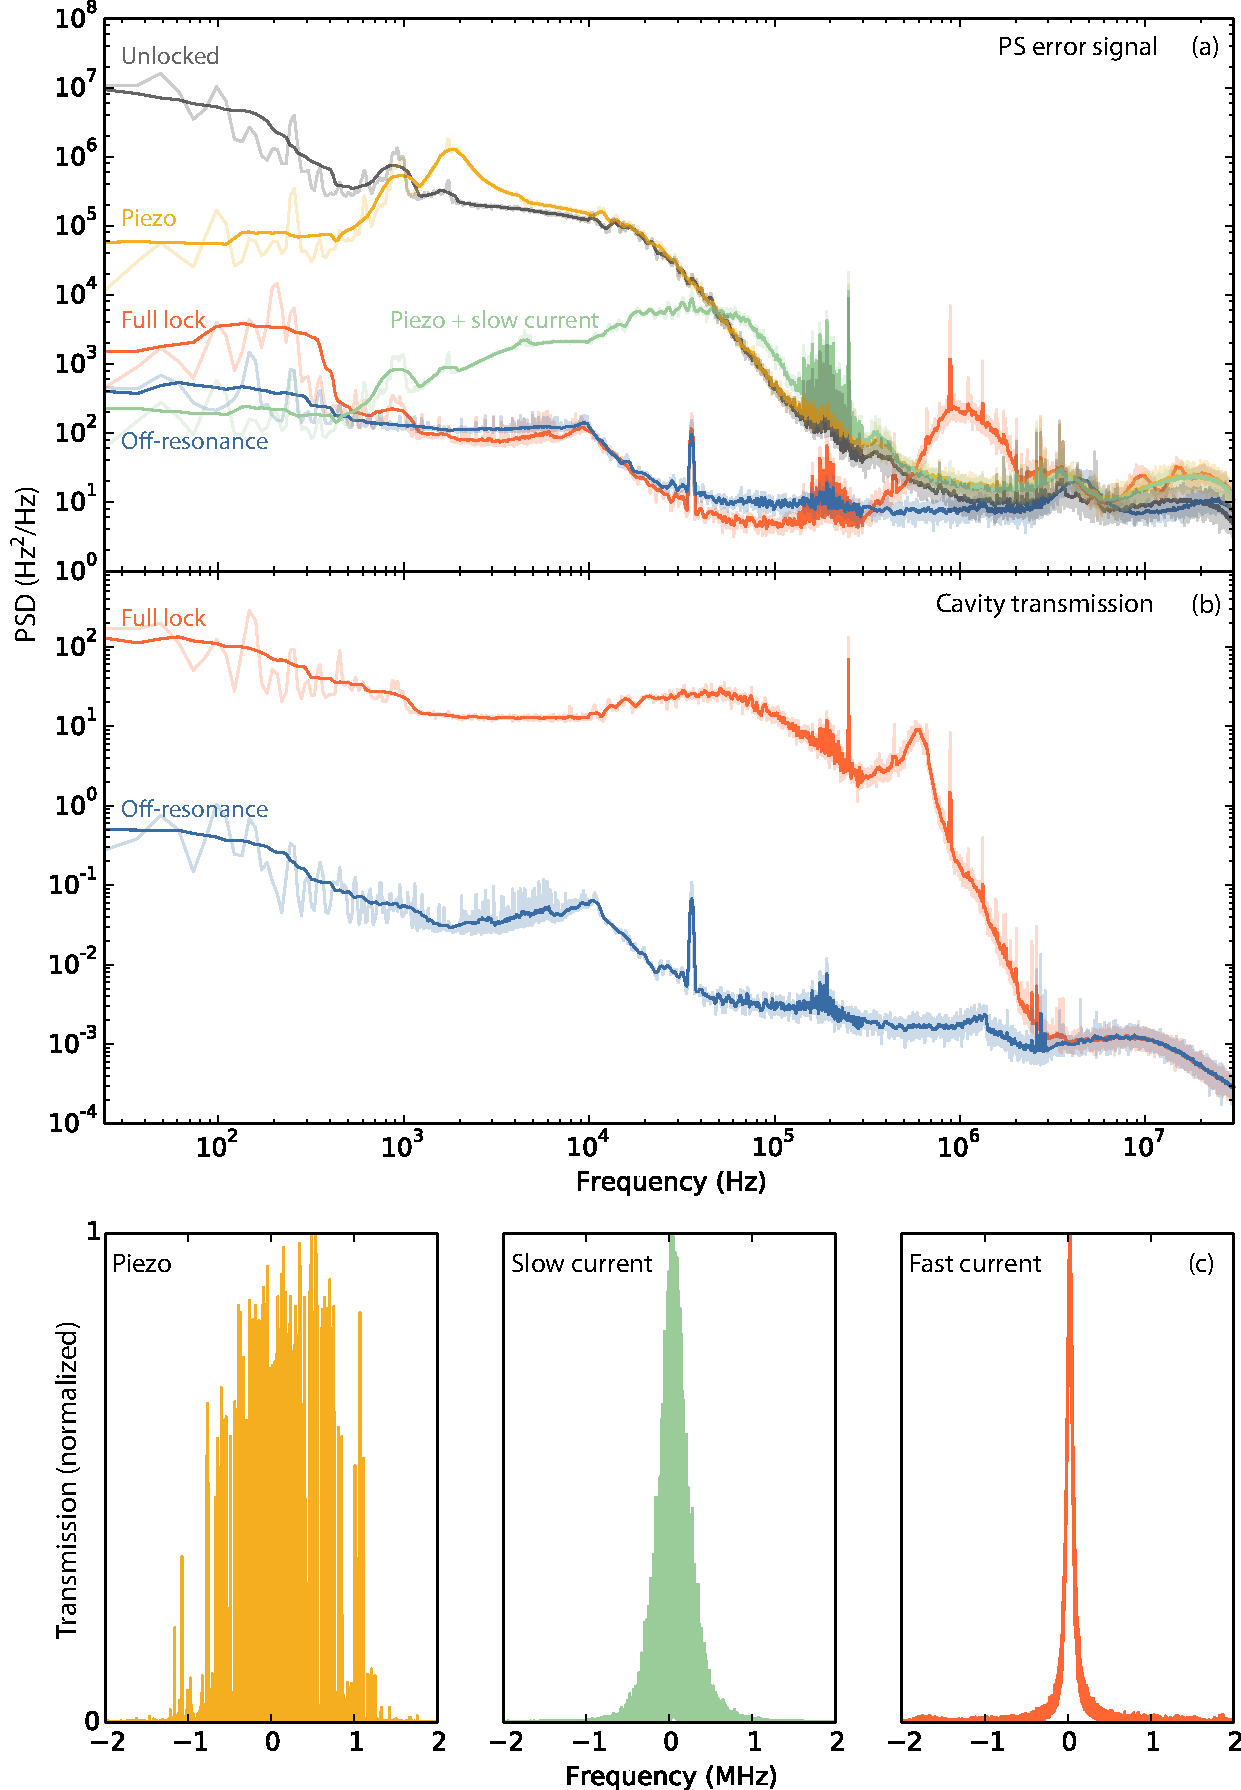
\includegraphics[width=0.9\linewidth]{scholten_fig3.pdf}
\caption{Frequency noise measurements.
(a) Power spectral density (PSD) of polarization spectroscopy (PS) error signals for a range of laser locking regimes with laser on resonance: unlocked; piezo-only feedback; slow current and piezo feedback; piezo, slow current, and fast AC-coupled current feedback; the noise floor of the noise measurement with the laser frequency off the atomic resonance.
Laser power 6.5\,mW after the stabilizing Glan-Thompson prism.
The measurements are shown with a superposed smoothed curve (moving average  with window size $10\log_{10}(f)$ where $f$ is the frequency).
(b) PSD of transmitted cavity signal at half peak height for the piezo, slow current and fast AC-coupled current feedback.
(c) Optical cavity transmission as a function of laser offset frequency for locking with varying bandwidth.
Piezo only (left), piezo and slow current (middle) and piezo, slow current and fast current (right).
Cavity FWHM linewidth 72\,kHz, scan time 100\,ms, laser power incident on the cavity $170\rm\,\mu W$.
For (a) and (b) noise below $10^4$\,Hz was measured with a high dynamic range audio digitizer with a resolution bandwidth (RBW) of 12\,Hz; a radio frequency spectrum analyzer was used at higher frequencies, with RBW of 30\,Hz between $10^4$\,Hz\textendash$10^6$\,Hz and RBW of 300\,Hz above $10^6$\,Hz.\label{fig:PSDs}\label{fig:cavity_scans}}
\end{figure}

\subsubsection{Error Signal Noise}
The frequency spectrum of the PS error signal provides a measure of laser frequency noise in combination with the PS frequency discrimination, photodetector and electronic noise and gain.
The response of the system to different feedback parameters and the underlying noise limitations are immediately apparent.
The frequency noise power spectral density (PSD) of the PS error signal (Fig.~\ref{fig:PSDs}a) was measured for different feedback configurations, using a high-dynamic-range audio digitizer (frequencies \textless10\,kHz) and radio frequency (RF) spectrum analyzer (frequencies, 10\,kHz to 30\,MHz).
The RF spectrum analyzer was calibrated using the slope of the error signal on resonance.
The low frequency data were calibrated by matching to the RF spectrum analyzer data at 10\,kHz.

Increasing suppression of noise is readily apparent as the feedback bandwidth is increased from 1\,kHz (piezo only) to 50\,kHz (piezo and slow current through the laser controller) and then full lock with feedback via direct diode current modulation.
From around 450\,Hz to 350\,kHz the fully locked noise spectrum is coincident with the noise floor (measured by detuning the laser far from resonance) and intersects with the unlocked spectrum at 700\,kHz.
The frequency of the servo bump at 1.3\,MHz is consistent with the phase lag in the laser diode response~\cite{wiemanhollberg}.

\subsubsection{Cavity Transmission Noise}
To measure the laser frequency noise spectrum we used a high-finesse optical cavity as an independent laser frequency discriminator~\cite{equipment}.
The optical cavity had finesse of $2.1\times 10^4$, free spectral range of 1.50\,GHz, and a FWHM linewidth of 72\,kHz.
Fig.~\ref{fig:cavity_scans}(c) shows cavity transmission signals as the laser frequency incident on the cavity was scanned with a double-pass acousto-optic modulator (AOM).
The resulting traces provide a clear illustration of the effect of increased locking bandwidth: with piezo-only locking the peak appears broad as the laser jitters around the resonant frequency.
With slow current feedback, the transmission peak shape becomes apparent, and finally we see the effect of high-bandwidth feedback with peak width limited by the cavity finesse, indicating a laser linewidth much smaller than the cavity linewidth.

We analyzed the frequency noise of the laser through the cavity transmission signal by choosing a static AOM frequency such that the transmitted power through the optical cavity was half the peak power, where the transmission-frequency response is approximately linear.
The cavity noise spectrum is shown in the lower portion of Fig.~\ref{fig:PSDs}(a) for full bandwidth AC-coupled locking.
The signal was well above the noise floor, measured with laser frequency between transmission peaks, for frequencies up to the 5.5\,MHz bandwidth of the photodetector.
This approach could not be used with lower-bandwidth feedback because the laser linewidth was wider than the cavity transmission.
Note that the cavity transmission noise floor is three to four orders of magnitude lower than that of the PS error signal, consistent with the lower shot noise in the cavity measurement where the laser power was $10\rm\,\mu$W compared to 1\,mW in the PS balanced polarimeter.

We extracted a measure of the linewidth from the cavity data using two methods: first we mapped the amplitude noise of the locked cavity signal to frequency using the cavity transmission frequency response shown in Fig.~\ref{fig:cavity_scans}(c).
The standard deviation of the distribution of frequencies gave a root mean square (RMS) linewidth of 2.4$\pm$0.3\,kHz.
We also integrated the cavity transmission signal PSD to find an RMS linewidth~\cite{negnevitsky_wideband_2013} of 2.4$\pm$0.7\,kHz.
Linewidth results are summarized in Table \ref{linewidth_table}.

The cavity transmission spectra and linewidth measurements include contributions from both laser frequency and amplitude noise.
An estimate of the amplitude noise contribution to the spectra was obtained by measuring the photodetector power spectrum without the cavity and thus without frequency noise, with the same incident laser power on the photodetector.
Mapping that noise spectrum to frequency produced a contribution of 1.4$\pm$0.2\,kHz in the cavity transmission mapping linewidth,  and 0.16$\pm$0.05\,kHz to the cavity PSD integral linewidth.
The inconsistency between these two measurements indicates that a large portion of the noise is at very low frequencies which are below the 24\,Hz PSD measurement cutoff.

Assuming the frequency and amplitude noise contributions are uncorrelated and that the observed signal is a convolution of the two indicates that the linewidth determined from the cavity transmission mapping consists of the 1.4$\pm$0.2\,kHz amplitude noise linewidth in combination with a frequency noise linewidth of 2.0$\pm$0.5\,kHz.
The inconsistency between the two linewidth measurements is probably due to the low frequency cutoff of the PSD measurement and the mapping method not properly including contributions from higher frequencies; that is, the ``pedestal'' of the laser spectrum which can be seen in a heterodyne measurement.

\subsection{Heterodyne Measurements}
To resolve the discrepancy between the two laser linewidth measurements we used heterodyne beatnotes, which are insensitive to amplitude noise.
Heterodyne measurements were made by frequency shifting one of the laser beams with a double-pass AOM and combining the two locked beams on a 50:50 beam splitter followed by a 1\,GHz bandwidth photodetector.
The beatnote spectrum was measured with an RF spectrum analyzer~\cite{equipment}, see Fig.~\ref{fig:beatnote}.
Most of the optical power was within the central peak of the spectrum, with $-3$\,dB full width of $2.0\pm0.4$\,kHz.
The lasers are uncorrelated and if they have identical Gaussian lineshapes then the single laser RMS linewidth was $0.60\pm0.1$\,kHz.
The shoulders in the spectrum around $\pm1.5$\,MHz correspond to the servo bump of the fully locked spectra in Fig.~\ref{fig:PSDs}(a).

The measurement shown inset in Fig.~\ref{fig:beatnote} is a 50-shot average with a total measurement time of approximately 2 seconds. Individual measurements had $-3$\,dB widths as low as 880$\pm$280\,Hz, corresponding to an RMS laser linewidth of 270$\pm$90\,Hz.

\begin{figure}[htbp]
\centering
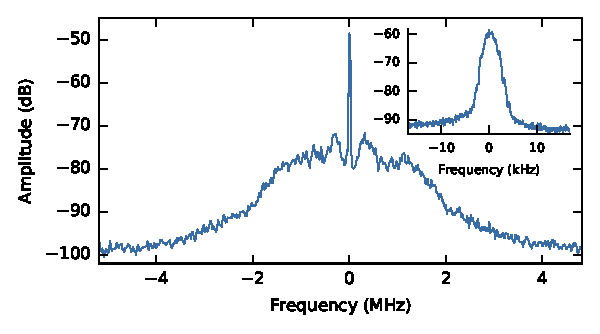
\includegraphics{scholten_fig4.pdf}
\caption{Heterodyne measurement for two lasers locked with polarization spectroscopy.
Inset: Higher resolution measurement of the central peak with $-3\rm\,dB$ width of 2.0$\pm$0.36\,kHz.
Both figures are 50 shot averages with resolution bandwidths of 30\,kHz and 100\,Hz and total measurement times of approximately 0.5\,s and 2\,s respectively.\label{fig:beatnote}}
\end{figure}

\begin{table}[htbp]
\centering
\begin{tabular}{c c c}
\hline
  & Method & RMS Linewidth (kHz) \\ \hline
  (i) & Cavity transmission mapping  & $2.0 \pm 0.5$ \\
  (ii) &Cavity transmission integral & $2.4 \pm 0.7$ \\
  (iii) & Heterodyne & $0.60\pm0.1$ \\ \hline\end{tabular}
\caption{Linewidth results.
(i) Mapping the transmission signal through a cavity with a FWHM of 72\,kHz to a Lorentzian signal followed by deconvolving from the amplitude noise.
(ii) The results from integrating the power-spectral density of the cavity transmission signal (Fig.~\ref{fig:PSDs}a).
(iii) Laser linewidth derived from the heterodyne measurement (Fig.~\ref{fig:beatnote}).}
\label{linewidth_table}
\end{table}

\subsection{Long-term Frequency Stability}
Polarization spectroscopy is inherently a DC technique, susceptible to low frequency drift ($1/f$ noise).
Drift in the laser power output as the laser alignment drifts, variations in fiber coupling efficiency if fibers are used, variations in the atomic vapor density due to changes in temperature, thermal effects on the waveplates and changes to the electronic gains and offsets can all affect the lock point of PS due to the resulting intensity noise combined with the difficulty in perfectly balancing the polarimeter.

The high-finesse cavity was used as a reference to quantify the long-term drift of the PS locked laser over a period of 60 hours (fig.~\ref{fig:drift}).
Drift in the optical cavity frequency was corrected by reference to a laser AC-locked to the rubidium transition using saturated absorption.
The standard deviation of the PS-locked laser frequency measurements was 51\,kHz, approximately half the standard deviation of the measurements in Ref.~\cite{tiwari_laser_2006} and significantly smaller than the 400\,kHz quoted in Ref.~\cite{lee_frequency_2014}.
The frequency change between 10\,s measurements was on average 5\,Hz, with a standard deviation of 210\,Hz.

\begin{figure}[htbp]
\centering
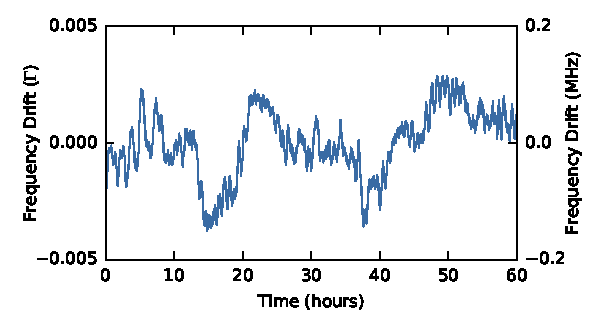
\includegraphics{scholten_fig5.pdf}
\caption{Frequency drift of a polarization spectroscopy locked laser, in units of natural linewidth $\Gamma$ and MHz, over a 60 hour period measured every 10 seconds.
The standard deviation of the frequency measurements was 51\,kHz.}
\label{fig:drift}
\end{figure}

The frequency stability of PS is strongly dependent on the extent to which the apparatus is isolated from ambient temperature variations~\cite{yoshikawa_frequency_2003}.
In our system the lasers are temperature stabilized and isolated with acrylic enclosures, and the optical cavity was temperature controlled and isolated inside a vacuum chamber, but the PS and SA components and optical components between lasers and optical cavity were not temperature controlled or shielded from the general laboratory environment.
The locking stability and drift are expected to improve with environmental isolation of all optical components and temperature stabilization of the atomic vapor cell.
The power into the PS setup is particularly sensitive to polarization drift in the light exiting the optical fibers.
Although singlemode polarization maintaining fibers were used, they exhibited significant polarization drift with laboratory temperature variations, and we expect shielded free-space propagation or active power stabilization of the light into the PS setup would further improve the frequency stability.


\section{Conclusion}

We have demonstrated laser frequency stabilization using a polarization spectroscopy reference, and reduced the linewidth of ECDL lasers well below 1\,kHz, much lower than previously demonstrated with this technique and previously achieved only by locking to high-finesse optical cavities.
The long-term frequency variance of 51\,kHz is sufficient for many laser cooling experiments and significantly lower than previously demonstrated.
Further improvements to drift can be expected with temperature stabilization and environmental isolation of the gas cells and fibers or replacing the fibers with free-space propagation.
The experimental setup provides an approach with low complexity and low cost, providing wide bandwidth linewidth narrowing without frequency modulation while retaining an absolute atomic reference.

\section{Acknowledgements}
We thank Andre Luiten for advice and equipment and Rory Speirs for confirmation of results.
BMS gratefully acknowledges the support of a University of Melbourne McKenzie Fellowship.
This work was supported by the Australian Research Council Linkage Project LP130100857.

\end{document}
